\documentclass[12pt]{article}

\usepackage{amsmath}
\usepackage{amssymb}
\usepackage{enumitem}
\usepackage[margin=1in]{geometry}
\usepackage{tikz}
\usetikzlibrary{
    arrows.meta,
    calc,
    angles,
    quotes,
    decorations.pathmorphing
}
\usepackage[american]{circuitikz}

\setlist[enumerate,1]{label=\arabic*.}
\setlist[enumerate,2]{label=\Alph*)}

\begin{document}

\begin{center}
\Large \textbf{Ultra-Hard Physics Paper (Single Correct MCQ)}
\end{center}

\vspace{0.5cm}

\begin{enumerate}

%=========================================================
%=========================================================
\item
A hollow conducting cube of side $a$ is placed in vacuum. 
A charge $\dfrac{q}{2}$ is located at the center of one face but slightly inside the cube, 
a charge $2q$ is located exactly at one vertex of the cube, 
and a charge $-q$ is placed at the geometric center of the cube. 

Considering correct fractional solid-angle sharing for boundary charges and induced charge redistribution on the inner surface, determine the net electric flux through the cube.

\begin{enumerate}
\item $-\dfrac{q}{4\varepsilon_0}$
\item $\dfrac{q}{4\varepsilon_0}$
\item $\dfrac{q}{2\varepsilon_0}$
\item zero
\end{enumerate}
%=========================================================
%=========================================================
%=========================================================
%=========================================================
\item
\textbf{(Ultra-Hard Magnetic Superposition Problem)}

An infinitely long straight wire carrying current $I$ is placed parallel to the $z$-axis at $x=a$.  
A circular loop of radius $R$ carrying current $I$ lies in the $xy$-plane centered at the origin.  

Determine the magnitude of the net magnetic field at the origin.

%---------------- Diagram ----------------
\begin{center}
\begin{tikzpicture}[scale=1]

% Axes
\draw[->] (-3,0) -- (3,0) node[right] {$x$};
\draw[->] (0,-3) -- (0,3) node[above] {$y$};

% Loop
\draw[thick] (0,0) circle (1.5);
\node at (1.8,0) {Loop $I$};

% Wire
\draw[thick] (2,-3) -- (2,3);
\node[right] at (2,2.5) {Wire $I$};

% Distance a
\draw[dashed] (0,0) -- (2,0);
\node at (1,-0.3) {$a$};

% Origin
\fill (0,0) circle (2pt);

\end{tikzpicture}
\end{center}

\begin{enumerate}
\item $\dfrac{\mu_0 I}{2R} + \dfrac{\mu_0 I}{2\pi a}$
\item $\left| \dfrac{\mu_0 I}{2R} - \dfrac{\mu_0 I}{2\pi a} \right|$
\item $\dfrac{\mu_0 I}{2R}$
\item $\dfrac{\mu_0 I}{2\pi a}$
\end{enumerate}
%=========================================================
%=========================================================
\item
An AC source $V_0 \sin \omega t$ is connected to a series $RLC$ circuit.
The frequency is adjusted so that the power factor becomes $\frac{1}{\sqrt{2}}$, and current leads voltage.

Determine the RMS current in steady state.

\begin{enumerate}
\item $\dfrac{V_0}{2R}$
\item $\dfrac{V_0}{\sqrt{2}R}$
\item $\dfrac{V_0}{\sqrt{2(R^2+(X_L-X_C)^2)}}$
\item $\dfrac{V_0}{R}$
\end{enumerate}

%=========================================================
\item
An electron in hydrogen atom is initially excited to $n=6$. It undergoes cascaded transitions emitting photons. Considering all possible transitions and selection rules ignored, determine the maximum possible photon energy and total number of distinct spectral lines possible.

\begin{enumerate}
\item $13.6\left(1-\frac{1}{36}\right), 15$
\item $13.6\left(1-\frac{1}{36}\right), 21$
\item $13.6\left(\frac{1}{1^2}-\frac{1}{6^2}\right), 15$
\item $13.6\left(\frac{1}{1^2}-\frac{1}{6^2}\right), 21$
\end{enumerate}

%=========================================================
%=========================================================
\item
\textbf{(Corrected Moving Slab Problem)}

A glass slab of thickness $t$ and refractive index $\mu$ moves with constant velocity $u$ parallel to its faces. A monochromatic ray is incident at angle $\theta$.

Using first-order relativistic velocity addition ($u \ll c$), determine the change in lateral displacement.

%---------------- Corrected Diagram ----------------
\begin{center}
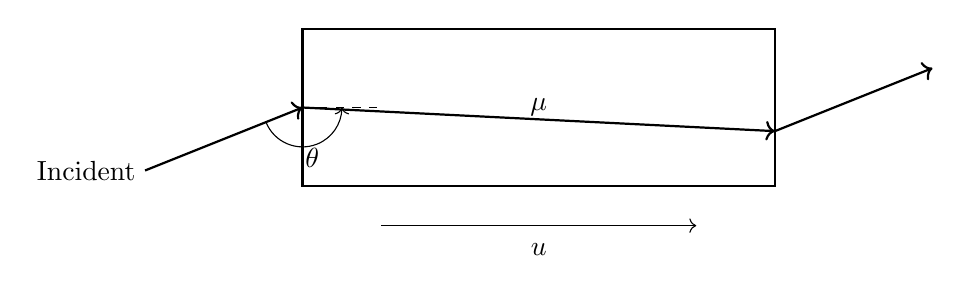
\begin{tikzpicture}[scale=1]

% Slab
\draw[thick] (-3,0) rectangle (3,2);
\node at (0,1) {$\mu$};

% Key coordinates
\coordinate (A) at (-5,0.2);   % incident start
\coordinate (B) at (-3,1);     % point of incidence
\coordinate (C) at (-2,1);     % normal direction

% Normal
\draw[dashed] (B) -- (C);

% Incident ray
\draw[->,thick] (A) -- (B);
\node[left] at (A) {Incident};

% Refracted inside
\draw[->,thick] (B) -- (3,0.7);

% Emergent
\draw[->,thick] (3,0.7) -- (5,1.5);

% Angle theta (correct: between incident ray and normal)
\pic[draw,->,"$\theta$",angle eccentricity=1.3]
{angle = A--B--C};

% Velocity
\draw[->] (-2,-0.5) -- (2,-0.5);
\node at (0,-0.8) {$u$};

\end{tikzpicture}
\end{center}

\begin{enumerate}
\item $\dfrac{ut}{c}\left(1-\dfrac{1}{\mu^2}\right)\tan\theta$
\item $\dfrac{ut}{\mu c}\tan\theta$
\item $\dfrac{ut}{c}\tan\theta$
\item zero change
\end{enumerate}

%=========================================================
%=========================================================


%=========================================================
\item
A block of mass $m$ attached to spring $k$ rests on rough surface with coefficient $\mu$. Initially compressed and released, motion involves stick-slip transitions near equilibrium. Determine minimum amplitude so that the block crosses equilibrium with nonzero speed after first half cycle.

\begin{enumerate}
\item $\dfrac{2\mu mg}{k}$
\item $\dfrac{3\mu mg}{k}$
\item $\dfrac{\mu mg}{k}$
\item $\dfrac{4\mu mg}{k}$
\end{enumerate}

%=========================================================
%=========================================================
\item
A solid sphere of radius $R$ rolls without slipping down an incline of length $L$ inclined at angle $\theta$. 
It then enters a horizontal rough surface where rolling resistance provides a constant retarding torque 
$\tau = \mu_r mgR$.

Determine the stopping distance on the horizontal surface.

%---------------- Diagram ----------------
\begin{center}
\begin{tikzpicture}[scale=1]

% Incline
\draw[thick] (-4,0) -- (0,2);

% Horizontal
\draw[thick] (0,2) -- (4,2);

% Sphere correctly touching incline
\draw[thick] (-2,1.4) circle (0.4);

% Angle
\draw (-3.5,0) arc (0:26:0.7);
\node at (-3.2,0.4) {$\theta$};

\node at (-2,2.1) {Sphere};

\end{tikzpicture}
\end{center}

\begin{enumerate}
\item $\dfrac{7L\sin\theta}{5\mu_r}$
\item $\dfrac{5L\sin\theta}{7\mu_r}$
\item $\dfrac{L\sin\theta}{\mu_r}$
\item $\dfrac{2L\sin\theta}{\mu_r}$
\end{enumerate}

%=========================================================
\item
A satellite moves in circular orbit of radius $R$. Due to small impulse tangentially, radius increases to $R+\Delta R$. Using first order Taylor expansion of orbital energy expression, determine fractional change in total mechanical energy.

\begin{enumerate}
\item $-\dfrac{\Delta R}{2R}$
\item $-\dfrac{\Delta R}{R}$
\item $\dfrac{\Delta R}{2R}$
\item $\dfrac{\Delta R}{R}$
\end{enumerate}

%=========================================================
\item
A rod fixed at both ends has temperature variation $\Delta T(x)=T_0(x/L)^3$. Considering compatibility condition and average strain zero, determine average thermal stress induced.

\begin{enumerate}
\item $\dfrac{E\alpha T_0}{4}$
\item $\dfrac{E\alpha T_0}{3}$
\item $\dfrac{E\alpha T_0}{2}$
\item $\dfrac{3E\alpha T_0}{4}$
\end{enumerate}

%=========================================================
\item
An ideal gas expands adiabatically from $V$ to $3V$. Using adiabatic relation and work integral, determine work done by gas in terms of initial pressure $P_0$.

\begin{enumerate}
\item $\dfrac{P_0V}{\gamma-1}(1-3^{1-\gamma})$
\item $P_0V(1-3^{1-\gamma})$
\item $\dfrac{P_0V}{\gamma}$
\item $3P_0V$
\end{enumerate}

%=========================================================
\item
A projectile is fired vertically upward with speed $u$. Considering time interval where kinetic energy exceeds potential energy, determine total duration satisfying inequality.

\begin{enumerate}
\item $\dfrac{u}{g}$
\item $\dfrac{u}{\sqrt{2}g}$
\item $\dfrac{\sqrt{2}u}{g}$
\item $\dfrac{2u}{g}$
\end{enumerate}

%=========================================================
%=========================================================
\item
\textbf{(Corrected Sliding Rod Problem)}

A conducting rod of length $L$ slides on frictionless U-shaped rails in a uniform magnetic field $B$ directed into the page. The rails are connected through a resistor $R$. The rod has mass $m$.

Determine the steady terminal velocity.

%---------------- Diagram ----------------
\begin{center}
\begin{circuitikz}[scale=1]

% Rails
\draw (0,0) -- (4,0);
\draw (0,3) -- (4,3);

% Rod
\draw[thick] (2,0) -- (2,3);
\node[right] at (2,1.5) {$L$};

% Resistor
\draw (4,3) to[R,l=$R$] (4,0);

% B field
\node at (1,1.5) {$\times$};
\node at (3,1.5) {$\times$};
\node at (2,2.5) {$B$};

% Motion arrow
\draw[->] (2,-0.5) -- (3,-0.5);
\node at (2.5,-0.8) {$v$};

\end{circuitikz}
\end{center}

\begin{enumerate}
\item $\dfrac{mgR}{B^2L^2}$
\item $\dfrac{mg}{BL}$
\item $\dfrac{mgR}{BL}$
\item $\dfrac{mg}{B^2L}$
\end{enumerate}

%=========================================================
%=========================================================
\item
\textbf{(Corrected Elastic Collision Problem)}

A particle of mass $m$ moving with speed $v$ collides elastically in one dimension with a stationary particle of mass $4m$.

Determine the final velocity of the first particle.

\begin{enumerate}
\item $-\dfrac{3v}{5}$
\item $-\dfrac{v}{5}$
\item $\dfrac{v}{5}$
\item $-\dfrac{2v}{5}$
\end{enumerate}

%=========================================================
%=========================================================
\item
\textbf{(Corrected YDSE Problem)}

In Young’s double slit experiment, one slit is covered with a thin glass plate introducing phase shift $\phi$. Simultaneously, the screen distance is doubled and the wavelength is halved.

Determine the new fringe width and shift of central maximum.

%---------------- Diagram ----------------
\begin{center}
\begin{tikzpicture}[scale=1]

% Slits
\draw[thick] (0,1) -- (0,2);
\draw[thick] (0,-1) -- (0,-2);

\node[left] at (0,1.5) {$S_1$};
\node[left] at (0,-1.5) {$S_2$};

% Glass
\draw[fill=gray!20] (0,1) rectangle (0.5,2);

% Screen
\draw[thick] (6,-3) -- (6,3);
\node at (6.5,0) {Screen};

% Axis
\draw[dotted] (0,0) -- (6,0);

\end{tikzpicture}
\end{center}

\begin{enumerate}
\item $\beta$, shift $=\dfrac{\phi}{2\pi}\beta$
\item $\beta/2$, shift $=\dfrac{\phi}{2\pi}\beta$
\item $2\beta$, shift doubled
\item $\beta$, no shift
\end{enumerate}
%=========================================================
\item
A solid non-conducting sphere of radius $R$ carries uniform volume charge density $\rho$. 
A smaller spherical cavity of radius $\dfrac{R}{2}$ is carved out such that its center is at a distance $\dfrac{R}{2}$ from the center of the original sphere.

Determine the magnitude of the electric field at the center of the cavity.

\begin{enumerate}
\item $\dfrac{\rho R}{6\varepsilon_0}$
\item $\dfrac{\rho R}{3\varepsilon_0}$
\item $\dfrac{\rho R}{4\varepsilon_0}$
\item zero
\end{enumerate}
%=========================================================

\end{enumerate}

\end{document}